% =============================================================================
%  Towards Autonomous Industrial Mobility:
%  An AI Framework for Optimal Path Planning and Resource-Efficient Navigation
%
%  Bachelor thesis — Arian Shafagh
%
%  Compile with pdfLaTeX + Biber (Overleaf: Menu -> Compiler -> pdfLaTeX).
%  Every chapter lives in its own file so chapters can be written, moved and
%  commented on independently:
%      preamble/  packages, styling, macros (numbers used in the text)
%      front/     title page, declaration, abstracts, acknowledgements
%      chapters/  the thesis itself, one file per chapter
%      back/      appendices
%      figures/   figures (the result figures are copied from tools/ai/results)
%      bib/       references.bib
% =============================================================================
\documentclass[a4paper,12pt,twoside,openright]{report}

% Packages. Keep this file boring: anything experimental belongs in style.tex.
\usepackage[T1]{fontenc}
\usepackage[utf8]{inputenc}
\usepackage[english]{babel}
\usepackage{lmodern}
\usepackage{microtype}
\usepackage{xspace}

\usepackage[a4paper,inner=3.2cm,outer=2.5cm,top=2.8cm,bottom=3.0cm]{geometry}
\usepackage{graphicx}
\graphicspath{{figures/}}
\usepackage{booktabs}          % \toprule \midrule \bottomrule — no vertical rules
\usepackage{tabularx}
\usepackage{multirow}
\usepackage{siunitx}           % \SI{8.42}{\watt\hour} — consistent units
\sisetup{per-mode=symbol, detect-weight=true}
\usepackage{amsmath,amssymb}
\usepackage{algorithm}
\usepackage{algpseudocode}
\usepackage{listings}          % code and YAML excerpts
\usepackage{caption}
\usepackage{subcaption}
\usepackage{enumitem}
\usepackage{xcolor}
\usepackage[hidelinks]{hyperref}
\usepackage[capitalise,noabbrev]{cleveref}

\usepackage[backend=biber,style=ieee,sorting=none,maxbibnames=6]{biblatex}

% Look and feel: headers, captions, code listings.
\usepackage{fancyhdr}
\pagestyle{fancy}
\fancyhf{}
\fancyhead[LE,RO]{\thepage}
\fancyhead[RE]{\nouppercase{\leftmark}}
\fancyhead[LO]{\nouppercase{\rightmark}}
\renewcommand{\headrulewidth}{0.4pt}

\captionsetup{font=small, labelfont=bf, margin=1em}
\setlength{\parskip}{0.3em}

\definecolor{codebg}{RGB}{247,247,245}
\definecolor{codekey}{RGB}{42,120,214}
\definecolor{codecomment}{RGB}{110,110,110}
\lstset{
  backgroundcolor=\color{codebg},
  basicstyle=\ttfamily\footnotesize,
  keywordstyle=\color{codekey},
  commentstyle=\color{codecomment}\itshape,
  breaklines=true,
  frame=single,
  rulecolor=\color{codebg},
  showstringspaces=false,
  captionpos=b,
  numbers=left,
  numberstyle=\tiny\color{codecomment},
}

% -----------------------------------------------------------------------------
% Numbers and names that appear many times. Defining them once means a value can
% never disagree with itself between chapters — and if a result is ever re-run,
% it is changed here, in one place.
% Sources: THESIS_DATA.md and HANDOVER.md in the repository root.
% -----------------------------------------------------------------------------

% --- policy names, so the thesis never mixes "NS" and "neuro-symbolic"
\newcommand{\NS}{neuro-symbolic model\xspace}
\newcommand{\NSshort}{NS\xspace}
\newcommand{\PPO}{PPO\xspace}

% --- headline results (fast simulator, 12 scenarios x 30 seeds = 3240 shifts)
\newcommand{\scoreNS}{53.81}
\newcommand{\scoreNSci}{[51.9,\,55.7]}
\newcommand{\scoreSymbolic}{52.91}
\newcommand{\scoreUnbounded}{51.56}
\newcommand{\scoreEstimateOnly}{52.85}
\newcommand{\scoreNeuralOnly}{51.81}
\newcommand{\scorePPO}{52.35}
\newcommand{\scoreRule}{41.66}
\newcommand{\scorePPOunmasked}{28.19}

% --- safety (shifts containing at least one violation, out of 360)
\newcommand{\violNS}{0/360}
\newcommand{\violPPO}{53/360}
\newcommand{\violNeuralOnly}{57/360}

% --- generalisation (the six scenarios written after training, 180 shifts each)
\newcommand{\unseenNS}{47.20}
\newcommand{\unseenSymbolic}{45.66}
\newcommand{\unseenPPO}{44.83}
\newcommand{\unseenUnbounded}{43.33}

% --- the heavy_load failure and its repair
\newcommand{\heavyUnbounded}{28.5}
\newcommand{\heavyBounded}{52.3}
\newcommand{\maxCorrection}{1.0}

% --- Gazebo validation
\newcommand{\gazeboEnergyGap}{+0.2\,\%}
\newcommand{\gazeboScoreGap}{-5.7\,\%}
\newcommand{\longShiftNS}{55.16}
\newcommand{\longShiftPPO}{37.79}
\newcommand{\longShiftNSbattery}{17.0\,\%}
\newcommand{\longShiftPPObattery}{9.4\,\%}

% --- planners
\newcommand{\thetaFaults}{6 of 17}
\newcommand{\navfnFaults}{0 of 5}

% --- shorthand for referring to the artefacts
\newcommand{\file}[1]{\texttt{#1}}


\addbibresource{bib/references.bib}

\begin{document}

% ------------------------------------------------------------------ front matter
\frontmatter
\begin{titlepage}
\centering
\vspace*{2cm}

{\Large \textsc{<University>}\par}
{\large <Faculty / Department>\par}

\vspace{2.5cm}
{\huge\bfseries Towards Autonomous Industrial Mobility\par}
\vspace{0.6cm}
{\LARGE An AI Framework for Optimal Path Planning\\and Resource-Efficient Navigation\par}

\vspace{2cm}
{\large Bachelor Thesis\par}
\vspace{0.4cm}
{\large in <degree programme>\par}

\vspace{2cm}
\begin{tabular}{rl}
Submitted by:   & Arian Shafagh\\
Matriculation number: & <number>\\
Supervisor:     & <name>\\
Second examiner:& <name>\\
Submission date:& <date>\\
\end{tabular}

\vfill
\end{titlepage}

\chapter*{Declaration of Authorship}
\addcontentsline{toc}{chapter}{Declaration of Authorship}

% Most universities prescribe the exact wording — replace this with your faculty's text.
I hereby declare that this thesis is my own work and that I have used no sources or aids other
than those stated. All passages taken from the literature, literally or in substance, are marked
as such. This thesis has not been submitted to any other examination authority.

% If your university requires a statement about AI tools, this is where it goes. Be factual:
% state which tool was used, for what (e.g. implementation support, analysis scripting), and that
% the scientific content, evaluation and conclusions are your own.

\vspace{2cm}
\noindent\rule{6cm}{0.4pt}\\
<Place>, <date> \hfill Arian Shafagh

\chapter*{Abstract}
\addcontentsline{toc}{chapter}{Abstract}

% ~250 words, and the only part of the thesis most people will read. One sentence per element:
%   1. Setting: one mobile robot serves three production sections in a maze-like factory.
%   2. Problem: what to do next is a decision under battery, heat and buffer-overflow constraints.
%   3. Approach: a neuro-symbolic policy (hard rules + priority tiers + a bounded neural ranker),
%      compared against masked PPO and two reference policies, in a fast simulator validated
%      against full ROS 2 / Gazebo shifts.
%   4. Result: score \scoreNS{} over 12 scenarios with \violNS{} safety violations, against
%      \scorePPO{} and \violPPO{} for PPO; and the Gazebo confirmation.
%   5. Contribution: the bound that keeps a learned ranker from overruling its own rules outside
%      the training distribution, and the sim-to-Gazebo validation of the energy model.

\textit{<abstract text>}

\vspace{1em}
\noindent\textbf{Keywords:} autonomous mobile robots, neuro-symbolic AI, deep reinforcement
learning, energy-aware navigation, ROS~2, Nav2, simulation.

% If your university requires a second abstract in another language, add it here as a
% \chapter*{Zusammenfassung} (or the appropriate heading).

\chapter*{Acknowledgements}
\addcontentsline{toc}{chapter}{Acknowledgements}

\textit{<optional; thank supervisors, reviewers, family. Keep it short and personal.>}


\tableofcontents
\listoffigures
\listoftables

% ---------------------------------------------------------------------- chapters
\mainmatter
\chapter{Introduction}
\label{ch:introduction}

% NARRATIVE GOAL OF THIS CHAPTER
% Make the reader care, then promise exactly what the thesis delivers. A bachelor thesis is
% judged partly on whether the question is clear by the end of page three.

\section{Motivation}
\label{sec:motivation}
% Industrial mobile robots move material between machines. The interesting decision is not "how do
% I drive there" (solved by navigation stacks) but "what is worth doing next": a full buffer stops
% a production line, a flat battery strands the robot, and every metre costs energy.
% Keep it concrete: the factory of this thesis produces 20, 30 and 5 units per hour in sections
% A, B and C; a buffer that fills is production lost for good.

\section{Problem statement}
\label{sec:problem-statement}
% One robot, three producing sections, one delivery point, one charger. A decision maker must pick
% the next action under hard constraints (battery reserve, motor temperature, payload, condition).
% Two families of answer exist: hand-written rules (predictable, but blind to trade-offs) and
% learned policies (good at trade-offs, but with no guarantee). This thesis asks whether the two
% can be combined so that the guarantee survives.

\section{Research questions}
\label{sec:research-questions}
% State them as questions you actually answer in \cref{ch:results}. Suggested:
\begin{enumerate}[label=\textbf{RQ\arabic*.}, leftmargin=*]
  \item \textit{<Does a neuro-symbolic policy outperform a deep reinforcement learning policy of
        equal information on throughput, energy and safety?>}
  \item \textit{<What does each half contribute — do the rules alone, or the network alone, suffice?>}
  \item \textit{<Do the policies still hold up in situations they were never trained on?>}
  \item \textit{<Do results obtained in a fast abstract simulator transfer to full physics
        simulation with a real navigation stack?>}
\end{enumerate}

\section{Contributions}
\label{sec:contributions}
% Be precise and modest; every item must be defensible with a number from \cref{ch:results}.
\begin{itemize}[leftmargin=*]
  \item A complete, reproducible ROS~2 system in which a single robot works an autonomous shift:
        factory model, energy/thermal/wear model, mission executor with recovery, decision service
        and a read-only monitor.
  \item A \NS whose hard rules can never be overruled, whose priority tiers are explicit, and whose
        learned ranker is \emph{bounded}: the correction it may apply is limited to
        $\pm\maxCorrection$ score units.
  \item The observation that motivates that bound: without it, the learned ranker carried a habit
        from its training scenarios into an overloaded factory it had never seen and waited while
        production lines stopped (\heavyUnbounded{} against \heavyBounded{} with the bound).
  \item An evaluation of 3240 simulated shifts with paired statistics and a held-out set of
        scenarios, validated by full Gazebo shifts in which the energy model agrees to
        \gazeboEnergyGap{}.
  \item A planner study showing that a global planner selected on short benchmark tours was the
        worse choice over full shifts (\thetaFaults{} shifts faulty against \navfnFaults{}).
\end{itemize}

\section{Outline}
\label{sec:outline}
% One or two sentences per chapter. Write this LAST, when the chapters exist.

\chapter{Background and Related Work}
\label{ch:background}

% NARRATIVE GOAL
% Two jobs: (1) teach the reader the few concepts they need, (2) show where this work sits and what
% gap it fills. Do not review the whole field — review what your argument needs.
% Source for citations: docs/related_work.md in the repository (20 verified peer-reviewed papers,
% 2024-2025, already grouped by the sections below; DOIs checked against Crossref).

\section{Autonomous mobile robots in production logistics}
\label{sec:amr}
% What AMRs do, why dispatching/task allocation matters, and the industrial framing.

\section{Navigation: ROS~2 and Nav2}
\label{sec:nav2}
% Only what the thesis uses: costmaps, global planners (NavFn, Theta*, Smac), a local controller
% (MPPI), AMCL localisation, behaviour trees and recovery. This sets up \cref{sec:planner-study}.

\section{Decision making for mobile robots}
\label{sec:decision-making}
\subsection{Rule-based and heuristic dispatching}
\subsection{Deep reinforcement learning}
% Policy-gradient methods, PPO, and action masking as the standard way to express legality.
\subsection{Neuro-symbolic approaches}
% Group A of docs/related_work.md. The closest peer-reviewed analogue keeps the symbolic part
% readable and editable after training; this thesis writes the symbolic part by hand instead,
% which is a difference to defend openly.

\section{Safety in learned policies}
\label{sec:safe-learning}
% Group B: shielding, action masking, constrained RL. The argument the results support: a mask
% expresses legality, but the guarantee comes from where the constraint is enforced.

\section{Energy-aware navigation and battery management}
\label{sec:energy-aware}
% Groups C and D: energy models, charge scheduling, and how energy consumption is calibrated —
% this justifies the parameters in \file{params.yaml} (\cref{app:configuration}).

\section{Simulation and sim-to-real validation}
\label{sec:sim2real}
% Group E: what is normally validated, and the gap this thesis addresses by comparing a fast
% abstract simulator against full Gazebo shifts.

\section{Research gap}
\label{sec:gap}
% Two or three sentences, sharp: existing work either learns the whole policy (no guarantee) or
% hand-writes it (no trade-off reasoning); reported evaluations rarely separate seen from unseen
% conditions; and abstract schedulers are seldom validated against a full navigation stack.

\chapter{Problem Setting}
\label{ch:problem}

% NARRATIVE GOAL
% Define the world precisely enough that a reader could rebuild it. Everything here is a fact of
% the setup, not a design decision of your solution — those belong in \cref{ch:system}.

\section{The factory}
\label{sec:factory}
% Layout (a 14.5 x 10 m maze hall), three sections A/B/C, one delivery point, one charger.
% Production rates 20, 30 and 5 units per hour; buffers of 8, 10 and 3 units; unit masses.
% Figure: the maze (thesis/figures/, e.g. a screenshot of the dashboard map or the Gazebo world).

\section{The robot}
\label{sec:robot}
% Differential drive, 0.39 m/s, 22 Wh battery, 15 % reserve, payload limit, motor temperature
% limit 70 C, wear. Table of parameters -> \cref{app:configuration}.

\section{Tasks and actions}
\label{sec:actions}
% The action vocabulary: PICKUP:<A|B|C>, DELIVER, CHARGE:<40|70|100>, WAIT:<s>. One action is one
% decision; the executor drives, dwells and reports.

\section{Objective}
\label{sec:objective}
% The single number everything is judged by, stated as an equation:
\begin{equation}
  \label{eq:objective}
  J = \underbrace{n_{\text{delivered}}}_{+1 \text{ each}}
    - \underbrace{n_{\text{lost}}}_{-1 \text{ each}}
    - 0.5\,\underbrace{E_{\text{battery}}}_{\si{\watt\hour}}
    - 20\,\underbrace{n_{\text{violations}}}_{\text{safety}}
\end{equation}
% Explain each weight and, honestly, what it does not count: idling on the charger is paid by the
% charger, not the battery (a limitation revisited in \cref{sec:limitations}).

\section{Constraints}
\label{sec:constraints}
% Battery reserve including the return trip, motor temperature, payload, maintenance condition.
% These are the constraints the symbolic layer enforces in \cref{sec:symbolic-layer}.

\section{Scenarios}
\label{sec:scenarios}
% 12 scenarios; six used for training, six written afterwards and never trained on. Table in
% \cref{app:scenarios}. Say clearly here that the split is what makes \cref{sec:generalisation}
% a generalisation result rather than a curve fit.

\chapter{System Design}
\label{ch:system}

% NARRATIVE GOAL
% Show that the platform is sound, so that the results in \cref{ch:results} can be trusted. Explain
% the decisions a reader would otherwise question ("why two simulators?", "why one node for all
% three sections?"). Source: HANDOVER.md, sections WP1-WP3 and WP7.

\section{Architecture overview}
\label{sec:architecture}
% One figure, drawn by you: layout.yaml -> generator -> {Gazebo world, Nav2 map, POIs, path
% matrix}; factory node; robot state node; mission executor; decision service; dashboard.
% Key principle to state explicitly: the decision layer never sees ROS, so the same policy object
% runs in the fast simulator and on the robot.

\section{One source of truth for the world}
\label{sec:single-source}
% layout.yaml is an ASCII grid; the generator emits the SDF world, the PGM map, the points of
% interest and the path-length matrix. Nothing can drift out of step.
% Worth telling as a story: the 0.5 m pinch that made Nav2 plan through a gap the robot could not
% pass, and the clearance check that now fails generation if such a gap exists (HANDOVER WP1).

\section{Factory model}
\label{sec:factory-model}
% Production as a Gamma process, buffers, BLOCKED/DEGRADED/FAULT states, seeded per section.

\section{Robot model: energy, heat and wear}
\label{sec:robot-model}
% Idle power, drive energy per metre, payload term, charging power, thermal and wear models.
% Mention the calibration error caught by a magnitude test (drive energy 3.6x too high, HANDOVER
% WP2) — it shows the model was checked, not assumed.

\section{Mission execution and recovery}
\label{sec:executor}
% Action -> navigation goal -> dwell -> report. The recovery ladder: retry, clear costmaps, back
% up, return to charger, declare stuck. The arrival check against AMCL that catches Nav2 reporting
% success at a blocked goal.

\section{Decision service and graceful degradation}
\label{sec:service}
% The policy runs as its own process; if it stops answering, the executor falls back to built-in
% rules and the shift continues. Report the measured decision latency (see \cref{sec:latency}).

\section{Monitoring}
\label{sec:monitoring}
% The read-only dashboard: section cards, robot state, decisions with their explanations, and the
% live maze map. Screenshot it for the thesis. Emphasise "read-only": the operator watches, the
% robot decides.

\section{Two simulators, and why}
\label{sec:two-simulators}
% Gazebo is physically faithful but real-time; the fast simulator runs a shift in milliseconds,
% which is what makes 3240 shifts and any training possible. The bridge between them is the
% validation in \cref{sec:gazebo-validation}: same models, same parameters, same objective.

\chapter{Decision Models}
\label{ch:models}

% NARRATIVE GOAL
% The core chapter. Build the model in the order a reader can follow: what the rules guarantee,
% what the network adds, and why the network must be kept on a leash.
% Source: HANDOVER.md WP5, WP6, WP9 and the WP9 follow-up.

\section{Overview}
\label{sec:model-overview}
% One figure: legal actions -> hard rules (forbid) -> priority tiers (rank) -> neural ranker
% (choose within the top tier) -> action + explanation string.

\section{The symbolic layer}
\label{sec:symbolic-layer}
\subsection{Hard rules}
% H1 maintenance, H2 payload, H3 battery reserve including the return trip (checked by simulating
% the route with the robot's own model), H4 motor temperature, H5 no pointless waiting.
% H5 is worth a paragraph of its own: it closes a gap between two thresholds, found only by
% watching a real shift (HANDOVER, WP9 follow-up).
\subsection{Priority tiers}
% Tier 2 unblock a stopped line, tier 1 prevent one from stopping, tier 0 routine.
\subsection{Explainability}
% Every decision carries the rules that fired. Quote one real explanation string from a log.

\section{The neural ranker}
\label{sec:neural-ranker}
\subsection{Features and the symbolic estimate}
% 27 features; the network learns a *residual* on an analytic estimate rather than the value
% itself. Say why: the estimate already captures the arithmetic, so the network only has to learn
% what the arithmetic misses.
\subsection{Training}
% Rollout look-ahead targets, policy iteration, a ranking loss (softmax cross-entropy per decision
% point) rather than regression, best-round selection on validation scenarios.
% The ranking loss was the decisive change — report it as such.

\section{Bounding the correction}
\label{sec:bounded-correction}
% THE contribution. Present it as a discovery, not as a design:
%   1. the unbounded model was worse than its own rules on unseen scenarios;
%   2. the trace showed it choosing WAIT while every line was blocked, with an explanation string
%      that said waiting only spends energy;
%   3. the cause: in training, production is half as fast and batching pays;
%   4. the fix: centre the correction on the candidates' mean and clip it to +-\maxCorrection;
%   5. the bound was chosen on TRAINING scenarios with validation seeds only (table of the sweep:
%      none 57.75, 20 -> 57.75, 10 -> 58.06, 5 -> 58.15, 2 -> 58.15, 1 -> 58.70, 0 -> 57.41).
% State the interpretation: the network may decide close calls, never overrule clear evidence.

\section{Reinforcement learning baseline}
\label{sec:ppo}
% MaskablePPO on the same environment, observation and reward. Training setup and the fairness fix
% (each parallel environment now draws a random training scenario, so all six are seen).
% The unmasked variant exists to ask how much of PPO's competence is simply knowing the rules.

\section{Reference policies and ablations}
\label{sec:ablations}
% rule (nearest section above 50 % buffer, charge when the reserve would break),
% ns_symbolic_only, ns_neural_only, ns_estimate_only, ns_unbounded, ppo_wp6.
% A table listing each policy and the exact question it answers is very effective here.

\chapter{Experimental Setup}
\label{ch:setup}

% NARRATIVE GOAL
% Convince the reader that the numbers in \cref{ch:results} mean what you say. Anyone who doubts a
% result should find the answer here.

\section{Evaluation protocol}
\label{sec:protocol}
% 9 policies x 12 scenarios x 30 seeds = 3240 shifts of one hour each. Every policy runs the SAME
% seeds, so every comparison is paired.

\section{Training and test separation}
\label{sec:splits}
% Test seeds start at 5000 and were never used for training or model selection (NS collection uses
% 12345+, NS round selection 1000-1003, PPO draws random seeds). Six scenarios were written after
% training and form the unseen set. Say why this matters: without it, "generalisation" is a claim,
% not a measurement.

\section{Metrics}
\label{sec:metrics}
% Score (\cref{eq:objective}), delivered units, lost production, energy (Wh and Wh per unit),
% charging trips, minimum battery, shifts containing a safety violation, decision latency.
% Define a "violation" exactly: battery below the reserve away from the charger, motor temperature
% at the limit, or an empty battery.

\section{Statistics}
\label{sec:statistics}
% 95 % bootstrap confidence intervals on the mean score (2000 resamples); paired Wilcoxon
% signed-rank tests against the \NS on identical seeds; significance level 0.05.
% Note honestly that no multiple-comparison correction is applied, and that with 30 paired seeds
% small differences can be significant without being important.

\section{Validation in Gazebo}
\label{sec:gazebo-setup}
% Full shifts through the real stack, then the same policy, scenario and seed replayed in the fast
% simulator. State the one subtlety: the executor finishes the action it has started when the
% shift ends, so the fast simulator is run in the same mode for comparison.

\section{Hardware and software}
\label{sec:hardware}
% ROS 2 Jazzy, Gazebo Harmonic 8.11 headless, Nav2 with MPPI, Python 3.12, PyTorch (CPU),
% Stable-Baselines3 / sb3-contrib. CPU, cores, RAM. Training times: PPO 9.8 min, NS ~40 min.

\chapter{Results}
\label{ch:results}

% NARRATIVE GOAL
% Report, do not yet interpret (interpretation is \cref{ch:discussion}). Every number here exists
% in THESIS_DATA.md; use the \newcommand macros from preamble/macros.tex so no value can drift.
% Tables: booktabs only, no vertical rules. Figures are in thesis/figures/.

\section{Overall comparison}
\label{sec:overall}
% Table: all nine policies, score with CI, delivered, lost, Wh, Wh/unit, shifts with a violation,
% delta against the \NS and the paired p-value. Numbers in preamble/macros.tex and
% tools/ai/results/summary_20260920_210847.md.

\begin{table}[htbp]
  \centering
  \caption{Shift score over all 12 scenarios (30 seeds each, 360 shifts per policy). Paired
           Wilcoxon signed-rank test against the \NS.}
  \label{tab:overall}
  \begin{tabular}{lrrrrr}
    \toprule
    Policy & Score [95\,\% CI] & \si{\watt\hour} & Shifts with violation & $\Delta$ & $p$\\
    \midrule
    \textbf{\NSshort{} (bounded)} & \textbf{\scoreNS{}} \scoreNSci{} & 8.42 & \textbf{\violNS{}} & --- & ---\\
    % ... fill the remaining rows from summary_20260920_210847.md
    \bottomrule
  \end{tabular}
\end{table}

\begin{figure}[htbp]
  \centering
  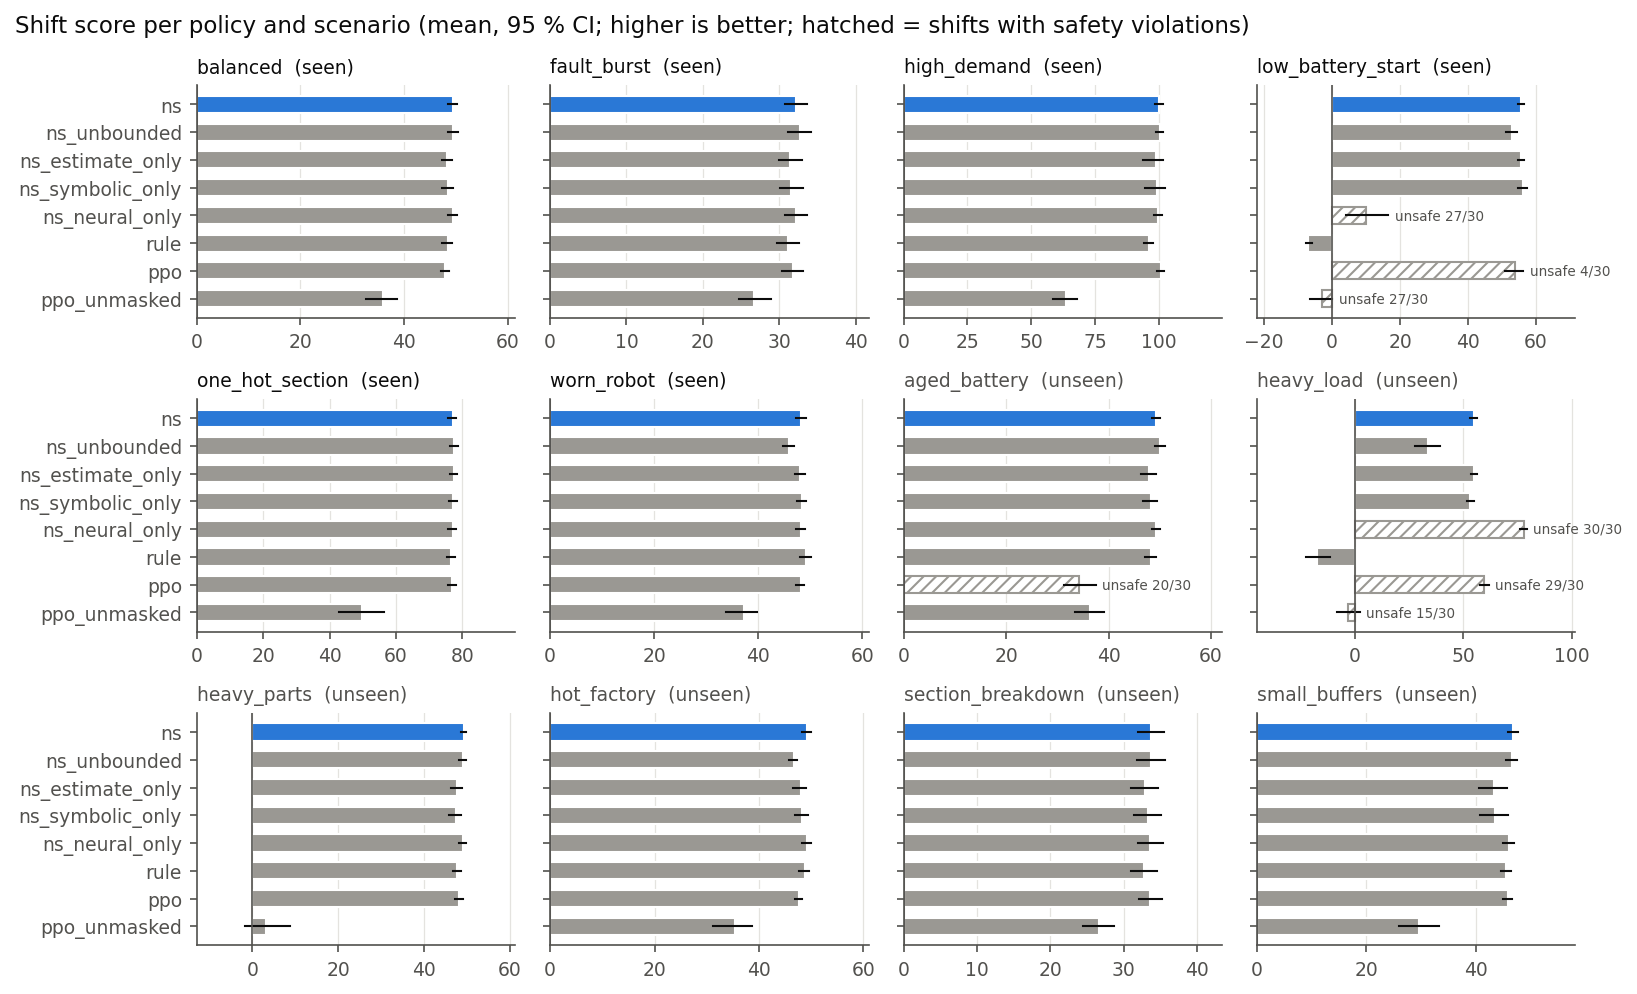
\includegraphics[width=\textwidth]{fig_score_by_scenario.png}
  \caption{Score per policy and scenario (mean, 95\,\% bootstrap CI). Hatched bars mark policies
           whose score includes shifts with safety violations.}
  \label{fig:score-by-scenario}
\end{figure}

\section{What each half contributes}
\label{sec:ablation-results}
% ns_symbolic_only \scoreSymbolic{}, ns_estimate_only \scoreEstimateOnly{}, ns_neural_only
% \scoreNeuralOnly{} (but \violNeuralOnly{} unsafe), ns_unbounded \scoreUnbounded{}.
% The sentence the chapter is built towards: the network helps only while it is bounded.

\section{Generalisation to unseen scenarios}
\label{sec:generalisation}
% \unseenNS{} against \unseenSymbolic{}, \unseenPPO{} and \unseenUnbounded{}; and the
% \heavyUnbounded{} -> \heavyBounded{} repair on heavy_load.

\section{Safety}
\label{sec:safety-results}
\begin{figure}[htbp]
  \centering
  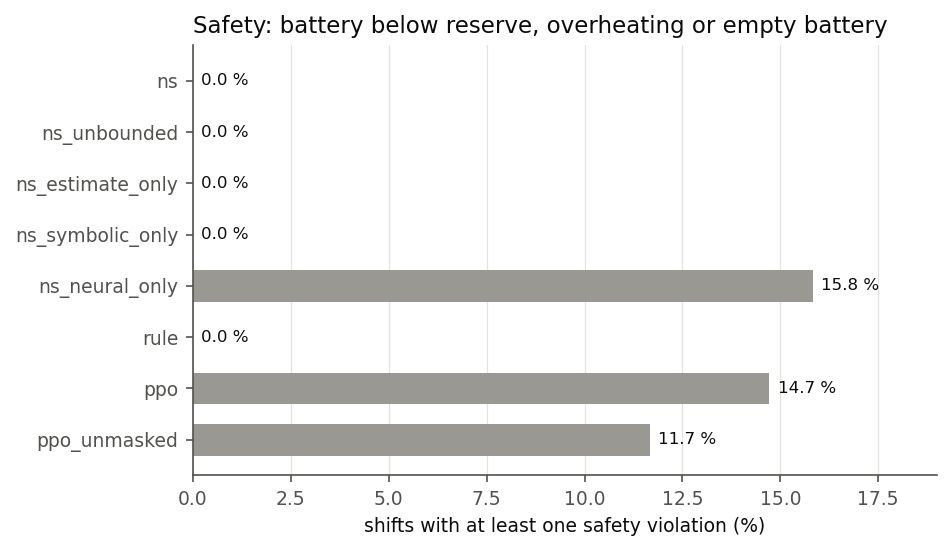
\includegraphics[width=0.8\textwidth]{fig_violations.png}
  \caption{Share of shifts containing at least one safety violation.}
  \label{fig:violations}
\end{figure}
% \violNS{} for every rule-carrying policy; \violPPO{} for PPO, of which 49 of 53 occur in unseen
% scenarios; \violNeuralOnly{} for the network without rules.

\section{Throughput and energy}
\label{sec:energy-results}
\begin{figure}[htbp]
  \centering
  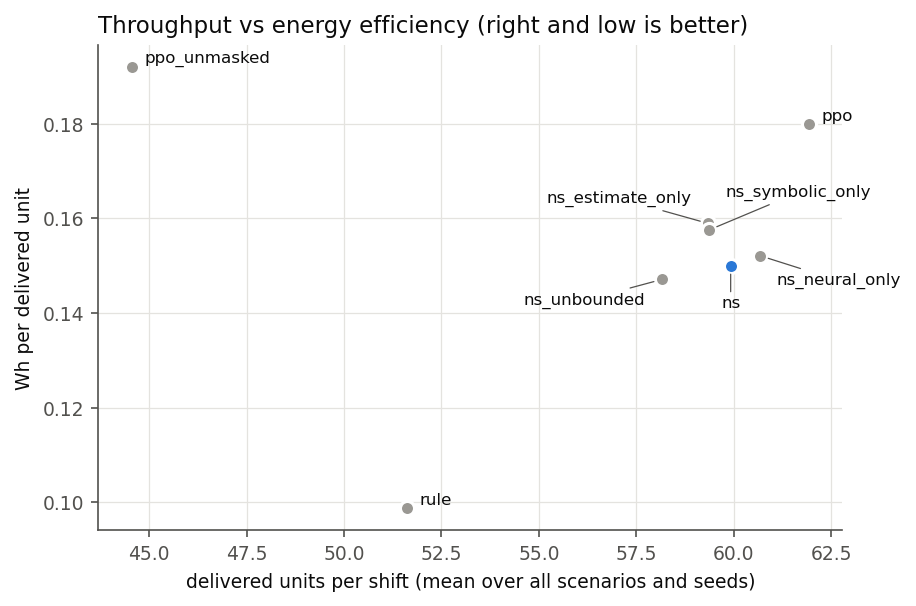
\includegraphics[width=0.75\textwidth]{fig_energy_throughput.png}
  \caption{Delivered units against energy per delivered unit, averaged over all scenarios.}
  \label{fig:energy-throughput}
\end{figure}
% PPO delivers slightly more but spends 10.21 Wh against 8.42 Wh and runs the battery lower.

\section{Decision latency}
\label{sec:latency}
% ~1.5 ms per decision for the \NS, comparable for PPO; irrelevant next to a 60 s action, which is
% the point worth making.

\section{Validation against Gazebo}
\label{sec:gazebo-validation}
\begin{figure}[htbp]
  \centering
  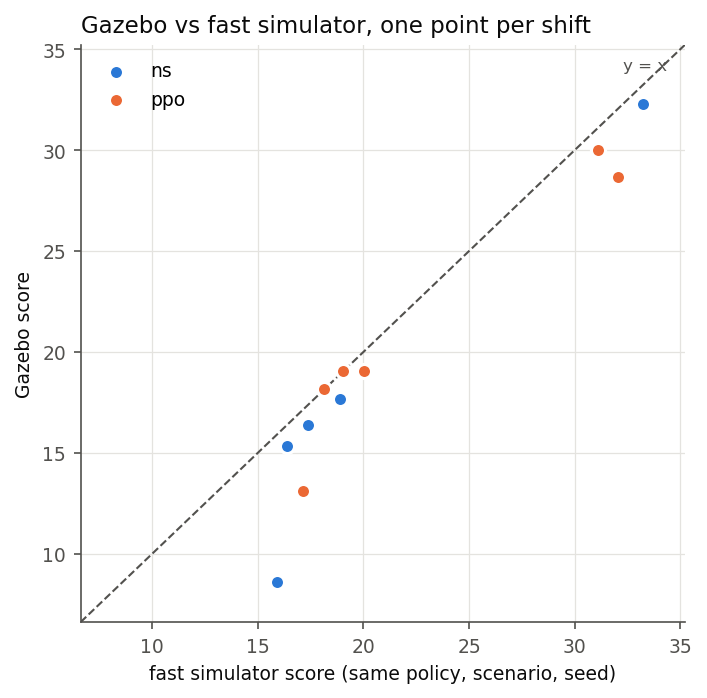
\includegraphics[width=0.62\textwidth]{fig_gazebo_vs_sim.png}
  \caption{Gazebo score against fast-simulator score for the same policy, scenario and seed.}
  \label{fig:gazebo-vs-sim}
\end{figure}
% 20-minute shifts: energy \gazeboEnergyGap{}, score \gazeboScoreGap{}, ranking unchanged.
% 60-minute shifts on low_battery_start: \NSshort{} \longShiftNS{} with a minimum battery of
% \longShiftNSbattery{}, PPO \longShiftPPO{} with \longShiftPPObattery{} and a below-reserve
% violation. This is the tier-1 safety finding reproduced with real navigation.

\section{Global path planner}
\label{sec:planner-study}
% Short tours (WP8): Theta* fastest, -3.3 % per tour, p = 0.001.
% Full shifts (WP9): Theta* faulty in \thetaFaults{} shifts, NavFn \navfnFaults{}, scores equal.
% Report the failure message verbatim -- it is the evidence for the mechanism.

\chapter{Discussion}
\label{ch:discussion}

% NARRATIVE GOAL
% Answer the research questions in order, say what the numbers mean, and be the first to name the
% weaknesses. Examiners reward a candidate who criticises their own work accurately.

\section{Answering the research questions}
\label{sec:answers}
% RQ1 ... RQ4, each in a short subsection or paragraph, each pointing at a table or figure.

\section{Why the bound works}
\label{sec:why-bound}
% The interpretation: the analytic estimate extrapolates (it is arithmetic on the current state),
% the network interpolates (it is a function fitted on a distribution). Bounding the network's
% influence keeps its judgement where it is reliable -- near-ties -- and lets the arithmetic decide
% when the evidence is clear. Relate this to shielding and masking in \cref{sec:safe-learning}:
% those constrain *legality*; the bound constrains *influence*.

\section{Why the rules matter more than the score}
\label{sec:rules-matter}
% PPO matches the \NS on score in seen scenarios but is unsafe in 14.7 % of shifts. Argue what a
% violation means in a real hall: a stranded robot, a stopped line, a person fetching it.

\section{Measurement decisions that changed conclusions}
\label{sec:measurement}
% Two honest stories worth telling, both of which changed a decision:
%   1. PPO had trained on only four of six scenarios; fixing it changed the comparison's fairness.
%   2. A planner chosen on short tours failed over full shifts. Benchmarks measure what they
%      measure, and the operating regime is part of the benchmark.

\section{Limitations}
\label{sec:limitations}
% Be specific and quantitative:
%   - the objective counts only battery energy, so idling on the charger is free in the score;
%   - one robot, one delivery point, one charger; no traffic, no human co-workers;
%   - the fast simulator abstracts driving into distance and time, and Gazebo validates that only
%     for the routes actually driven;
%   - the 60-minute Gazebo comparison is one shift per model, a demonstration rather than a
%     statistic;
%   - the symbolic layer is hand-written and therefore only as good as its author's understanding;
%   - simulation throughout: no physical robot.

\section{Threats to validity}
\label{sec:validity}
% Internal: seeds, paired tests, no multiple-comparison correction.
% External: one layout, one robot model, one objective weighting.
% Construct: does the score really express what a factory wants? What would change with different
% weights (the ratio of energy cost to a lost unit is the interesting one)?

\chapter{Conclusion and Future Work}
\label{ch:conclusion}

\section{Conclusion}
\label{sec:conclusion}
% Half a page. What was built, what was measured, what the answer is. No new facts, no citations.
% The single sentence a reader should leave with: a learned ranker improves a rule-based policy
% only while it cannot overrule the rules -- and the improvement survives in full simulation.

\section{Future work}
\label{sec:future-work}
% Grounded in what this thesis actually leaves open (see the open issues in HANDOVER.md), not a
% wish list:
%   - count charging energy in the objective and re-train both models;
%   - learn the bound, or make it state-dependent (wide where the network is well supported,
%     narrow where it is not);
%   - the batching trade-off seen in worn_robot: a longer rollout horizon during training;
%   - several robots and a shared charger, which turns this into a scheduling problem;
%   - a physical robot, where localisation error and unmodelled friction test the energy model;
%   - a learned symbolic layer (rule induction) instead of a hand-written one.


% ------------------------------------------------------------------- back matter
\printbibliography[heading=bibintoc]

\appendix
\chapter{Configuration Parameters}
\label{app:configuration}

% The full parameter set from src/robofetch_factory/config/params.yaml: battery 22 Wh, reserve
% 15 %, idle power, drive energy per metre, payload term, thermal and wear constants, objective
% weights, the neuro-symbolic settings (urgency horizon, safety margin, max_correction 1.0) and
% the PPO hyper-parameters. Present as tables, or include the file verbatim with \lstinputlisting.

\chapter{Scenarios}
\label{app:scenarios}

% Table of the 12 scenarios: name, seen/unseen, one-line description, and what it stresses
% (overload, faults, heat, small buffers, aged battery, ...). The descriptions are in
% src/robofetch_factory/config/scenarios/*.yaml.

\chapter{Reproducing the Results}
\label{app:reproduction}

% The commands that produce every number in \cref{ch:results}, so the work is reproducible:
%   venv/bin/python tools/ai/evaluate.py --policies all --workers 10
%   venv/bin/python tools/ai/plot_results.py --episodes ... --gazebo ...
%   venv/bin/python -u tools/ai/run_gazebo_batch.py --models ns ppo --scenarios ... --shift-min 60
%   ./scripts/run.sh          (interactive: scenario, model, planner, view, shift length)
% Plus the repository URL and the commit hash of the version that produced the results.


\end{document}
